\documentclass[a4paper,12pt]{article}
\usepackage{graphicx, geometry, subfigure, amsmath, adjustbox, array}
\geometry{a4paper,left=2cm,right=2cm,top=1cm,bottom=2cm}
\setlength{\baselineskip}{12pt}
\renewcommand\arraystretch{1.5}
\renewcommand{\d}{\mathrm{d}}
\newcommand{\cm}{\mathrm{cm}}
\newcommand{\s}{\mathrm{s}}
\newcommand{\g}{\mathrm{g}}

\title{\textbf{Stars and Planets Problem Set3}}
\author{Qingru Hu}
\date{\today}

\begin{document}
\maketitle
\section*{\textbf{Exercise \uppercase\expandafter{\romannumeral3}.1  Energetics of collapsing clouds}}
\section*{(a)}
The eccentricity, semi-major axis and the orbital period of a particle that starts from $r=R$ and 
collapses towards the center is relatively $e=1$, $a=R/2$ and $T=2t_{\text{ff}}$. From the Kelper 
third law we have:
\begin{equation*}
    \frac{T^2}{a^3} = \frac{4\pi^2}{GM}
\end{equation*}
Therefore, the free-fall time is:
\begin{equation*}
    t_{\text{ff}} = \frac{1}{2} \sqrt{\frac{4\pi^2 a^3}{G M}} 
    = \frac{1}{2} \sqrt{\frac{4\pi^2 (\frac{R}{2})^3}{G \rho \frac{4\pi}{3} R^3}}
    = \sqrt{\frac{3\pi}{32 G\rho}}
\end{equation*}

\section*{(b)}
The Jeans Mass is:
\begin{equation*}
    M_\text{J} = (\frac{5kT}{G\mu m_\text{u}})^{\frac{3}{2}} (\frac{3}{4\pi \rho})^{\frac{1}{2}}
\end{equation*}
Substitute $\rho = \frac{M_\text{J}}{\frac{4\pi}{3} R^3_\text{J}}$ and we get:
\begin{equation*}
    R_{\text{J}} = \frac{G\mu m_\text{u}}{5kT} M_\text{J}
\end{equation*}

\section*{(c)}
According to the Virial Theorem, When the gas cloud collapses, half of its gravitational energy 
is radiated and the other half goes into the internal energy.
\begin{equation*}
    L = -\frac{\d E}{\d t} = \frac{\d U_{\text{int}}}{\d t} =-\frac{1}{2} \frac{\d W}{\d t}
\end{equation*}
We have assumed that during fragmentation, the temperature of the cloud remains constant, so the 
increase in the internal energy from the gravitational energy is also radiated away. That is to say, 
during the isothermal fragmentation, all the gravitational energy of the cloud is turned into radiation. 
Therefore, it is fair enough to estimate the radiation rate of the fragment to be all of its gravitational 
energy $\frac{GM^2}{R}$ divided by the free-fall time $t_{\text{ff}}$.
\begin{equation*}
    \frac{\d E}{\d t} \sim \frac{GM^2}{Rt_{\text{ff}}}
\end{equation*}
For a fragment that has $M = M_{\text{M}}$ and $R = R_{\text{J}}$, the radiation rate is approximately:
\begin{equation*}
    \frac{\d E}{\d t} = \frac{2\sqrt{2}}{\pi G} (\frac{5kT}{\mu m_{\text{u}}})^{\frac{5}{2}}
\end{equation*}

\section*{(d)}
The maximum rate that objects can cool by black body radiation is given by the Stefan-Boltzmann law:
\begin{equation*}
    \frac{\d E_{\text{cool}}}{\d t} = 4\pi R^2 \sigma T^4 
\end{equation*}
Pulge in the relation of $R_\text{J}$ and $M_\text{J}$ we have got in (b):
\begin{equation*}
    \frac{\d E_{\text{cool}}}{\d t} = 4\pi \sigma (\frac{G\mu m_\text{u}}{5k})^2 M_\text{J}^2 T^2
\end{equation*}

\section*{(e)}
\begin{figure}[htbp]
    \centering
    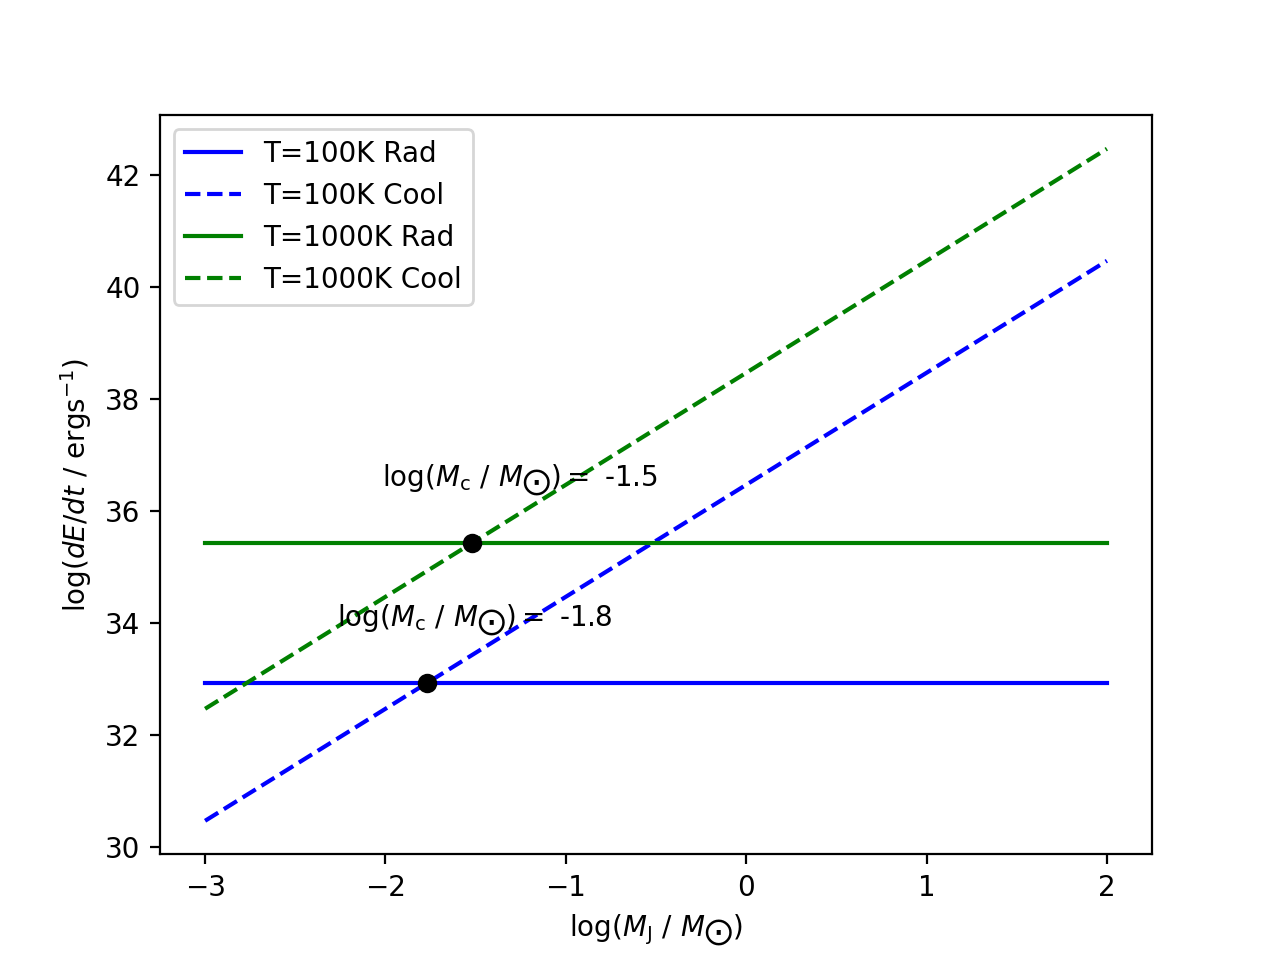
\includegraphics[width=10cm]{frag.png}
    % \caption{The relation}
\end{figure}

\section*{(f)}
Fragmentation stops at this point because if the Jeans Mass gets further smaller, 
the rate of radiation will be greater than the rate of cooling. When the rate of radiation 
is greater than the rate of cooling, cooling becomes uneffective and 
heat will be trapped, transforming the process from isothermal to adiabatic and 
increasing the Jeans Mass. With the Jeans Mass increased, the fragmentation stops.

\end{document}
